\documentclass[12pt]{article}
\usepackage[letterpaper, portrait, margin=1in]{geometry}
\usepackage{amsmath, amsfonts, amssymb, blkarray, tikz, colortbl}
\usepackage[normalem]{ulem}
\usetikzlibrary{arrows}

\tikzset{
  treenode/.style = {align=center, inner sep=0pt, text centered,
    font=\sffamily},
  arn_n/.style = {treenode, circle, black, font=\sffamily\bfseries, draw=black,
    fill=white, text width=0.8cm}}

\newcommand{\ques}[1]{\noindent {\bf Question #1: }} 

\setlength\parindent{0pt}

\usepackage{fancyhdr}
\pagestyle{fancy}
\fancyhf{}
\lhead{Darshan Patel}
\rhead{Data Mining}
\renewcommand{\footrulewidth}{0.4pt}
\cfoot{\thepage}

\begin{document}

\begin{center} \textbf{Assignment 5} \end{center}

\ques{1} Consider a dataset for frequent set mining as in the following table where we have $6$ binary features and each row represents a transaction. 
$$ \begin{matrix} & I1 & I2 & I3 & I4 & I5 & I6 \\ T1 & 0 & 0 & 1 & 0 & 1 & 0 \\ T2 & 0 & 1 & 1 & 1 & 0 & 1 \\ T3 & 1 & 0 & 0 & 0 & 1 & 0 \\ T4 & 1 & 1 & 1 & 0 & 0 & 0 \\ T5 & 0 & 0 & 0 & 1 & 0 & 0 \\ T6 & 1 & 0 & 0 & 1 & 0 & 1 \\ T7 & 0 & 0 & 1 & 1 & 1 & 1 \\ T8 & 1 & 0 & 1 & 0 & 1 & 0 \\ T9 & 1 & 0 & 0 & 1 & 0 & 0 \\ T10 & 0 & 1 & 1 & 0 & 0 & 1 \end{matrix} $$ 
\begin{enumerate} 
\item Illustrate the first three levels of the Apriori algorithm (set sizes $1$, $2$ and $3$) for support threshold of $3$ transactions, by identifying candidate sets and calculating their support. What are the maximal frequent sets discovered in the first $3$ levels? \\
For the first scan, C1 is $$ \begin{tabular}{|c|c|} \hline 
Transactions & Items \\ \hline 
T1 & \{I3, I5\} \\ \hline T2 & \{I2, I3, I4, I6\} \\ \hline
T3 & \{I1, I5\} \\ \hline T4 & \{I1, I2, I3\} \\ \hline 
T5 & \{I4\} \\ \hline T6 & \{I1, I4, I6\} \\ \hline 
T7 & \{I3, I4, I5, I6\} \\ \hline T8 & \{I1, I3, I5\} \\ \hline 
T9 & \{I1, I4\} \\ \hline T10 & \{I2, I3, I6\} \\ \hline \end{tabular} $$ 
Therefore L1 is $$ \begin{tabular}{|c|c|c|c|c|c|c|} \hline 
Items & I1 & I2 & I3 & I4 & I5 & I6 \\ \hline 
Count & 5 & 3 & 6 & 5 & 4 & 4 \\ \hline \end{tabular} $$ 
For the second scan, C2 is $$ \begin{tabular}{|c|c|} \hline 
Items & Count \\ \hline 
\{I1, I2\} & 1 \\ \hline \{I1, I3\} & 2 \\ \hline \{I1, I4\} & 2 \\ \hline \{I1, I5\} & 2 \\ \hline \{I1, I6\} & 1 \\ \hline \{I2, I3\} & 3 \\ \hline \{I2, I4\} & 1 \\ \hline \{I2, I5\} & 0 \\ \hline \{I2, I6\} & 2 \\ \hline \{I3, I4\} & 2 \\ \hline \{I3, I5\} & 3 \\ \hline \{I3, I6\} & 3 \\ \hline \{I4, I5\} & 1 \\ \hline \{I4, I6\} & 3 \\ \hline \{I5, I6\} & 1 \\ \hline \end{tabular} $$ 
Therefore L2 is $$ \begin{tabular}{|c|c|c|c|c|} \hline 
Items & \{I2, I3\} & \{I3, I5\} & \{I3, I6\} & \{I4, I6\} \\ \hline 
Count & 3 & 3 & 3 & 3 \\ \hline \end{tabular} $$ 
For the third scan, C3 is $$ \begin{tabular}{|c|c|} \hline 
Transactions & Items \\ \hline 
\{I2, I3, I4\} & 1 \\ \hline 
\{I2, I3, I5\} & 0 \\ \hline 
\{I2, I3, I6\} & 2 \\ \hline 
\{I3, I5, I6\} & 1 \\ \hline \end{tabular} $$ 
Note that no count is $3$ or more; therefore there are no items in L3. 

\item Pick one of the maximal sets and check if any of its subsets are association rules with frequency at least $0.3$ and confidence at least $0.6$. Explain your answer and show all work. \\
Pick the first row from L2, or $\{I2, I3\}$. Its count is $3$. The count of $I2$ and $I3$ is $3$ and $6$, respectively. Then the association rule for $I2 \to I3$ is
$$\text{confidence} =  \frac{\text{count of I2 and I3}}{\text{count of I2}} = \frac{3}{3} = 1 $$ 
and for $I3 \to I2$ is $$\text{confidence} =  \frac{\text{count of I2 and I3}}{\text{count of I3}} = \frac{3}{6} = 0.5 $$ 
Since only the confidence of $I2$ is greater than the minimum confidence of $0.6$, only $I2 \to I3$ is an association rule. 

\end{enumerate} 

\ques{2} Given the following transaction database, let the min\_support = $2$. 
$$ \begin{tabular}{|c|c|} \hline 
TID & Items \\ \hline 
1 & \{a,b,e\} \\ \hline 
2 & \{a,b,c,d\} \\ \hline 
3 & \{a,c,d\} \\ \hline 
4 & \{a,c,e\} \\ \hline 
5 & \{b,c,f\} \\ \hline
6 & \{a\} \\ \hline 
7 & \{a,b,c\} \\ \hline 
8 & \{b,d,e\} \\ \hline 
9 & \{a,c\} \\ \hline 
10 & \{a,b,d,e\} \\ \hline \end{tabular} $$ 
\begin{enumerate} 
\item Construct FP-tree from the transaction database. \\
Counts: 
$$ \begin{tabular}{|c|c|c|c|c|c|}  \hline
a & b & c & d & e & f \\ \hline 
8 & 6 & 6 & 4 & 4 & 1 \\ \hline \end{tabular} $$ 
Remove f since min\_support = $2$. 
$$ 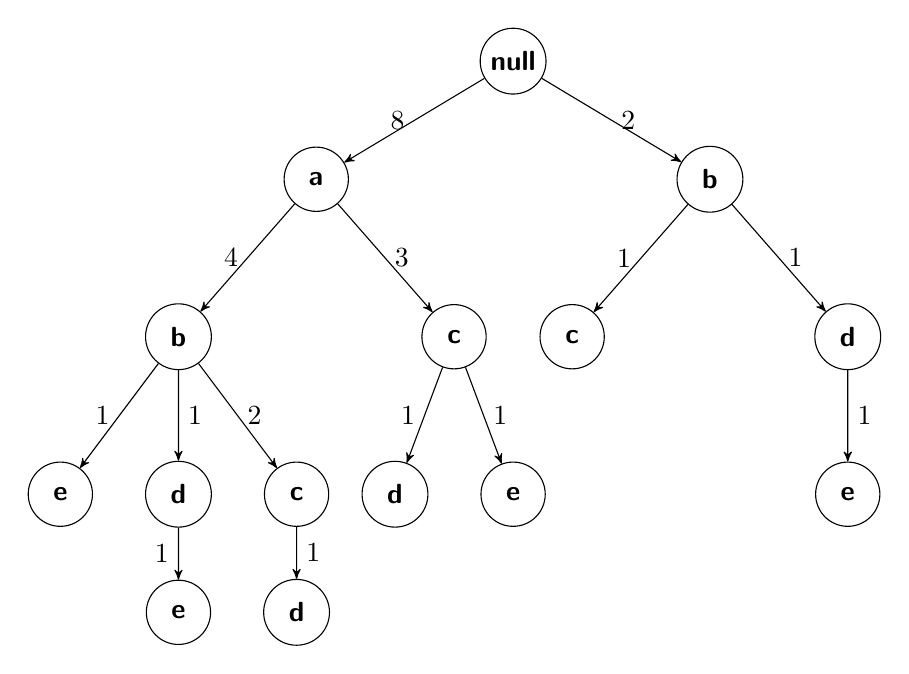
\begin{tikzpicture}[->,>=stealth',level/.style={sibling distance = 5cm/#1,
  level distance = 1.5cm}]
 \tikzstyle{level 2}=[sibling distance=35mm, level distance = 20mm] 
 \tikzstyle{level 3}=[sibling distance=15mm, level distance = 20mm] 
 
\node [arn_n] {null}
	child{ node [arn_n] {a}
		child{ node [arn_n] {b}
			child{ node [arn_n] {e}
				edge from parent node [left] {$1$} }
			child {node [arn_n] {d} 
				child {node [arn_n] {e}
					edge from parent node [left] {$1$} }
				edge from parent node [right] {$1$} }
			child{ node [arn_n] {c}
				child{ node [arn_n] {d}
					edge from parent node [right] {$1$} }
				edge from parent node [right] {$2$} }
			edge from parent node[left] {$4$} }
		child{ node [arn_n] {c}
			child{ node [arn_n] {d}
				edge from parent node [left] {$1$} }
			child{ node [arn_n] {e}
				edge from parent node [right] {$1$} }
			edge from parent node[right] {$3$} }
		edge from parent node[left] {$8$}}
	child{ node [arn_n] {b}
		child{ node [arn_n] {c}
			edge from parent node[left] {$1$} }
		child{ node [arn_n] {d}
			child{ node [arn_n] {e}
				edge from parent node[right] {$1$} }
			edge from parent node[right] {$1$} }
		edge from parent node[right] {$2$}}
; 
\end{tikzpicture} $$ 

\item Show d's conditional pattern base (projected database), d's conditional FP-tree and find frequent patterns based on d's conditional FP-tree. \\
d's Conditional Pattern Base: 
$$ \begin{tabular}{|c|c|c|c|} \hline
ab & ac & abc & b \\ \hline
1 & 1 & 1 & 1 \\ \hline \end{tabular} $$ 
 d's Conditional FP-tree: 
$$ 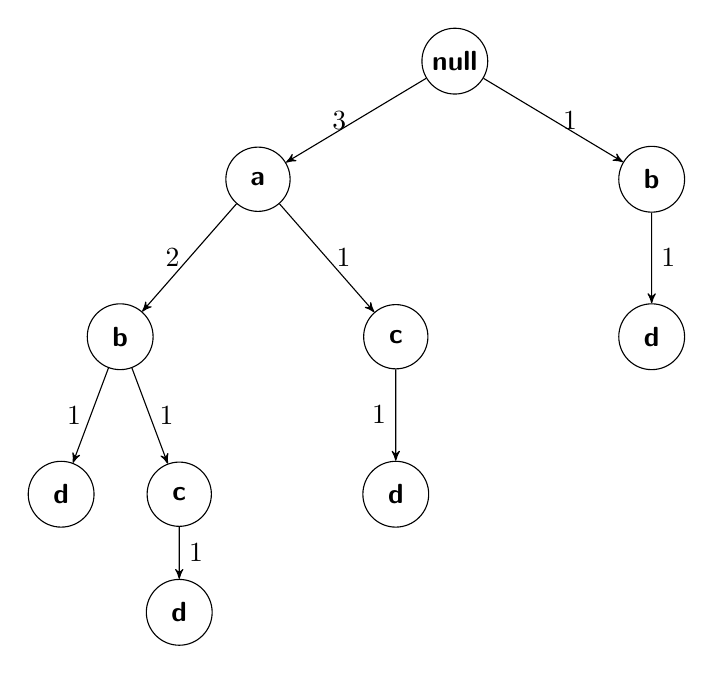
\begin{tikzpicture}[->,>=stealth',level/.style={sibling distance = 5cm/#1,
  level distance = 1.5cm}]
 \tikzstyle{level 2}=[sibling distance=35mm, level distance = 20mm] 
 \tikzstyle{level 3}=[sibling distance=15mm, level distance = 20mm] 
 
\node [arn_n] {null}
	child{ node [arn_n] {a}
		child{ node [arn_n] {b}
			child {node [arn_n] {d} 
				edge from parent node [left] {$1$} }
			child{ node [arn_n] {c}
				child{ node [arn_n] {d}
					edge from parent node [right] {$1$} }
				edge from parent node [right] {$1$} }
			edge from parent node[left] {$2$} }
		child{ node [arn_n] {c}
			child{ node [arn_n] {d}
				edge from parent node [left] {$1$} }
			edge from parent node[right] {$1$} }
		edge from parent node[left] {$3$}}
	child{ node [arn_n] {b}
		child{ node [arn_n] {d}
			edge from parent node[right] {$1$} }
		edge from parent node[right] {$1$}}
; 
\end{tikzpicture} $$ 
Remove d from the FP-tree and then look at Prefix trees. \\
$$ \begin{tikzpicture}[->,>=stealth',level/.style={sibling distance = 5cm/#1,
  level distance = 1.5cm}]
 \tikzstyle{level 2}=[sibling distance=35mm, level distance = 20mm] 
 \tikzstyle{level 3}=[sibling distance=15mm, level distance = 20mm] 
 
\node [arn_n] {null}
	child{ node [arn_n] {a}
		child{ node [arn_n] {b}
			child{ node [arn_n] {c}
				edge from parent node [right] {$1$} }
			edge from parent node[left] {$2$} }
		child{ node [arn_n] {c}
			edge from parent node[right] {$1$} }
		edge from parent node[left] {$3$}}
	child{ node [arn_n] {b}
		edge from parent node[right] {$1$}}
; 
\end{tikzpicture} $$ Found: ad, bd, cd since $a = 3 \geq 2$, $b = 2 \geq 2$ and $c = 2 \geq 2$.

For ``ad": 
$$ 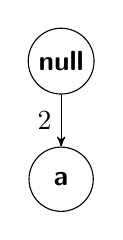
\begin{tikzpicture}[->,>=stealth',level/.style={sibling distance = 5cm/#1,
  level distance = 1.5cm}]
 \tikzstyle{level 2}=[sibling distance=35mm, level distance = 20mm] 
 \tikzstyle{level 3}=[sibling distance=15mm, level distance = 20mm] 
 
\node [arn_n] {null}
	child{ node [arn_n] {a}
			edge from parent node[left] {$2$} } 
; 
\end{tikzpicture} $$ None found because a is in highest order and ad is found. 

For ``bd": 
$$ 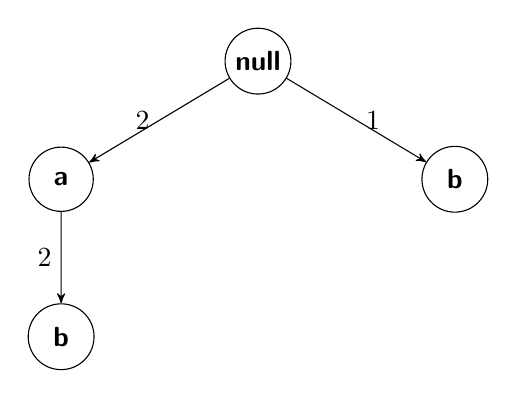
\begin{tikzpicture}[->,>=stealth',level/.style={sibling distance = 5cm/#1,
  level distance = 1.5cm}]
 \tikzstyle{level 2}=[sibling distance=35mm, level distance = 20mm] 
 \tikzstyle{level 3}=[sibling distance=15mm, level distance = 20mm] 
 
\node [arn_n] {null}
	child{ node [arn_n] {a}
		child{ node [arn_n] {b}
			edge from parent node[left] {$2$} }
		edge from parent node[left] {$2$}}
	child{ node [arn_n] {b}
		edge from parent node[right] {$1$}}
; 
\end{tikzpicture} $$ to
$$ 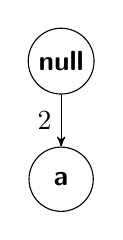
\begin{tikzpicture}[->,>=stealth',level/.style={sibling distance = 5cm/#1,
  level distance = 1.5cm}]
 \tikzstyle{level 2}=[sibling distance=35mm, level distance = 20mm] 
 \tikzstyle{level 3}=[sibling distance=15mm, level distance = 20mm] 
 
\node [arn_n] {null}
	child{ node [arn_n] {a}
		edge from parent node[left] {$2$}} 
; 
\end{tikzpicture} $$ Found: abd since $b = 2 \geq 2$. 

For ``cd":
$$ 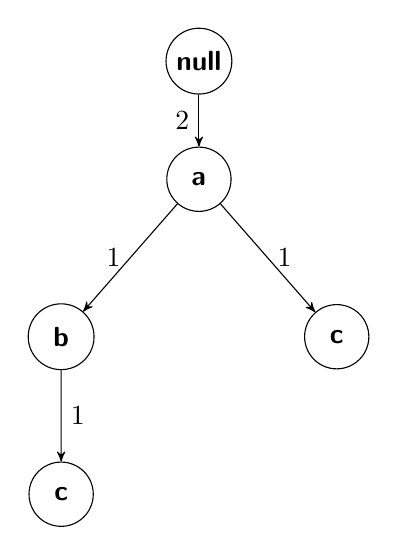
\begin{tikzpicture}[->,>=stealth',level/.style={sibling distance = 5cm/#1,
  level distance = 1.5cm}]
 \tikzstyle{level 2}=[sibling distance=35mm, level distance = 20mm] 
 \tikzstyle{level 3}=[sibling distance=15mm, level distance = 20mm] 
 
\node [arn_n] {null}
	child{ node [arn_n] {a}
		child{ node [arn_n] {b}
			child{ node [arn_n] {c}
				edge from parent node [right] {$1$} }
			edge from parent node[left] {$1$} }
		child{ node [arn_n] {c}
			edge from parent node[right] {$1$} }
		edge from parent node[left] {$2$}}
; 
\end{tikzpicture} $$ to
$$ 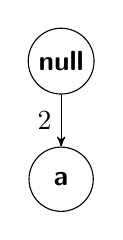
\begin{tikzpicture}[->,>=stealth',level/.style={sibling distance = 5cm/#1,
  level distance = 1.5cm}]
 \tikzstyle{level 2}=[sibling distance=35mm, level distance = 20mm] 
 \tikzstyle{level 3}=[sibling distance=15mm, level distance = 20mm] 
 
\node [arn_n] {null}
	child{ node [arn_n] {a}
		edge from parent node[left] {$2$}}
; 
\end{tikzpicture} $$ Found acd since $a = 2 \geq 2$. \\~\\ 
All frequent item set for d's condition FP-tree: 
\begin{center} ad, bd, cd, abd, acd \end{center}

\end{enumerate} \newpage

\ques{3} In the GSP algorithm, suppose the length-$3$ frequent pattern set $L_3$ is
$$\text{Row 1: } \langle \{2\}~\{3\}~\{4\} \rangle $$ 
$$\text{Row 2: }  \langle \{2~5 \}~\{3\} \rangle $$ 
$$\text{Row 3: } \langle \{3\}~\{4\}~\{5\} \rangle $$ 
$$\text{Row 4: } \langle \{1\}~\{2\}~\{3\} \rangle $$ 
$$\text{Row 5: } \langle \{1\}~\{2~5\} \rangle $$ 
$$\text{Row 6: } \langle \{1\}~\{5\}~\{3\} \rangle $$ 
$$\text{Row 7: } \langle \{5\}~\{3~4\} \rangle $$ 
Generate length-$4$ candidates set $C_4$ and frequent pattern set $L_4$. Show all work by writing down the details of the joins and prune steps. \\
For the first step, for each row set, drop the first element and compare it to the other row sets whose last element is dropped. \\
For Row 1, look for $\langle\{3\}~\{4\}\rangle$: 
$$ \begin{tabular}{|c|} \hline 
 \sout{$\langle \{2\}~\{3\}~\{4\} \rangle$} \\ \hline 
 $\langle \{2~5 \}~\{3\} \rangle$ \\ \hline 
 $\checkmark~\langle \{3\}~\{4\}~\{5\} \rangle$ \\ \hline
 $\langle \{1\}~\{2\}~\{3\} \rangle$ \\ \hline
 $\langle \{1\}~\{2~5\} \rangle$ \\ \hline 
 $\langle \{1\}~\{5\}~\{3\} \rangle$ \\ \hline 
 $\langle \{5\}~\{3~4\} \rangle$ \\ \hline \end{tabular} $$ Set 3.
 
 For Row 2, look for $\langle\{5\}~\{3\}\rangle$: 
$$ \begin{tabular}{|c|} \hline 
 $\langle \{2\}~\{3\}~\{4\} \rangle$ \\ \hline 
 \sout{$\langle \{2~5 \}~\{3\} \rangle$} \\ \hline 
 $\langle \{3\}~\{4\}~\{5\} \rangle$ \\ \hline
 $\langle \{1\}~\{2\}~\{3\} \rangle$ \\ \hline
 $\langle \{1\}~\{2~5\} \rangle$ \\ \hline 
 $\langle \{1\}~\{5\}~\{3\} \rangle$ \\ \hline 
 $\checkmark~\langle \{5\}~\{3~4\} \rangle$ \\ \hline \end{tabular} $$ Set 7. 

 For Row 3, look for $\langle\{4\}~\{5\}\rangle$: 
$$ \begin{tabular}{|c|} \hline 
 $\langle \{2\}~\{3\}~\{4\} \rangle$ \\ \hline 
 $\langle \{2~5 \}~\{3\} \rangle$ \\ \hline 
 \sout{$\langle \{3\}~\{4\}~\{5\} \rangle$} \\ \hline
 $\langle \{1\}~\{2\}~\{3\} \rangle$ \\ \hline
 $\langle \{1\}~\{2~5\} \rangle$ \\ \hline 
 $\langle \{1\}~\{5\}~\{3\} \rangle$ \\ \hline 
 $\langle \{5\}~\{3~4\} \rangle$ \\ \hline \end{tabular} $$ None Found.
 
 For Row 4, look for $\langle\{2\}~\{3\}\rangle$: 
$$ \begin{tabular}{|c|} \hline 
 $\checkmark~\langle \{2\}~\{3\}~\{4\} \rangle$ \\ \hline 
 $\langle \{2~5 \}~\{3\} \rangle$ \\ \hline 
 $\langle \{3\}~\{4\}~\{5\} \rangle$ \\ \hline
 \sout{$\langle \{1\}~\{2\}~\{3\} \rangle$} \\ \hline
 $\langle \{1\}~\{2~5\} \rangle$ \\ \hline 
 $\langle \{1\}~\{5\}~\{3\} \rangle$ \\ \hline 
 $\langle \{5\}~\{3~4\} \rangle$ \\ \hline \end{tabular} $$ Set 1. 
 
 For Row 5, look for $\langle\{2 ~ 5\}\rangle$: 
$$ \begin{tabular}{|c|} \hline 
 $\langle \{2\}~\{3\}~\{4\} \rangle$ \\ \hline 
 $\checkmark~\langle \{2~5 \}~\{3\} \rangle$ \\ \hline 
 $\langle \{3\}~\{4\}~\{5\} \rangle$ \\ \hline
 $\langle \{1\}~\{2\}~\{3\} \rangle$ \\ \hline
 \sout{$\langle \{1\}~\{2~5\} \rangle$} \\ \hline 
 $\langle \{1\}~\{5\}~\{3\} \rangle$ \\ \hline 
 $\langle \{5\}~\{3~4\} \rangle$ \\ \hline \end{tabular} $$ Set 2. 
 
 For Row 6, look for $\langle\{5\}~\{3\}\rangle$: 
$$ \begin{tabular}{|c|} \hline 
 $\langle \{2\}~\{3\}~\{4\} \rangle$ \\ \hline 
 $\langle \{2~5 \}~\{3\} \rangle$ \\ \hline 
 $\langle \{3\}~\{4\}~\{5\} \rangle$ \\ \hline
 $\langle \{1\}~\{2\}~\{3\} \rangle$ \\ \hline
 $\langle \{1\}~\{2~5\} \rangle$ \\ \hline 
 \sout{$\langle \{1\}~\{5\}~\{3\} \rangle$} \\ \hline 
 $\checkmark~\langle \{5\}~\{3~4\} \rangle$ \\ \hline \end{tabular} $$ Set 7. 
 
 For Row 7, look for $\langle\{3 ~ 4\}\rangle$: 
$$ \begin{tabular}{|c|} \hline 
 $\langle \{2\}~\{3\}~\{4\} \rangle$ \\ \hline 
 $\langle \{2~5 \}~\{3\} \rangle$ \\ \hline 
 $\checkmark~\langle \{3\}~\{4\}~\{5\} \rangle$ \\ \hline
 $\langle \{1\}~\{2\}~\{3\} \rangle$ \\ \hline
 $\langle \{1\}~\{2~5\} \rangle$ \\ \hline 
 $\langle \{1\}~\{5\}~\{3\} \rangle$ \\ \hline 
 \sout{$\langle \{5\}~\{3~4\} \rangle$} \\ \hline \end{tabular} $$ Set 3. \\~\\
 Therefore the length-$4$ candidates set $C4$ is 
 $$ \begin{tabular}{|c|} \hline 
 Row 1: $ \langle \{2\}~\{3\}~\{4\}~\{5\} \rangle $ \\ \hline
 Row 2: $ \langle \{2~5\}~\{3~4\} \rangle $ \\ \hline 
 Row 3: $ \langle \{1\}~\{2\}~\{3\}~\{4\} \rangle $ \\ \hline 
 Row 4: $ \langle \{1\}~\{2~5\}~\{3\} \rangle $ \\ \hline 
 Row 5: $ \langle \{1\}~\{5\}~\{3\}~\{4\} \rangle $ \\ \hline 
 Row 6: $ \langle \{5\}~\{3~4\}~\{5\} \rangle $ \\ \hline \end{tabular} $$ 
 
 To prune, check if subsequences of above candidates are in L3. If all of a certain candidates' subsequences exist in L3, put it in L4, the length-$4$ frequent pattern set. \\
 For Row 1: the subsequences are $$ \langle \{3\}~\{4\}~\{5\} \rangle,~ \langle \{2\}~\{4\}~\{5\} \rangle, ~ \langle \{2\}~\{3\}~\{5\} \rangle, ~ \langle \{2\}~\{3\}~\{4\} \rangle $$ of which only the first and last exist in L3. \\
 For Row 2: the subsequences are $$ \langle \{5\}~\{3~4\} \rangle, ~\langle \{2\}~\{3~4\} \rangle,~ \langle\{2~5\}~\{4\}\rangle,~\langle\{2~5\}~\{3\}\rangle $$ of which only the first, second, and fourth exist in L3. \\
 For Row 3, the subsequences are $$ \langle \{2\}~\{3\}~\{4\}\rangle,~\langle \{1\}~\{3\}~\{4\}\rangle,~ \langle\{1\}~\{2\}~\{4\}\rangle, ~\langle\{1\}~\{2\}~\{3\}\rangle $$ of which only the first and last exist in L3. \\ 
 For Row 4, the subsequences are $$ \langle\{2~5\}~\{3\}\rangle, \langle\{1\}~\{5\}~\{3\}\rangle,~\langle\{1\}~\{2\}~\{3\}\rangle,~\langle\{1\}~\{2~5\}\rangle $$ of which all four subsequences exist in L3. Remove this row from L4. \\
 For Row 5, the subsequences are $$ \langle\{5\}~\{3\}~\{4\}\rangle,~\langle\{1\}~\{3\}~\{4\}\rangle,~\langle\{1\}~\{5\}~\{4\}\rangle,~\langle\{1\}~\{5\}~\{3\}\rangle $$ of which only the first and last exist in L3. \\
 For Row 6, the subsequences are $$ \langle\{3~4\}~\{5\}\rangle,~\langle\{5\}~\{4\}~\{5\}\rangle,~\langle\{5\}~\{3\}~\{5\}\rangle,~\langle\{5\}~\{3~4\}\rangle $$ of which only the first and last exist in L3. \\~\\
 Therefore, $$ \begin{tabular}{|c|} \hline C4 \\ \hline 
 $ \langle \{2\}~\{3\}~\{4\}~\{5\} \rangle $ \\ \hline
 $ \langle \{2~5\}~\{3~4\} \rangle $ \\ \hline 
 $ \langle \{1\}~\{2\}~\{3\}~\{4\} \rangle $ \\ \hline 
 $ \langle \{1\}~\{5\}~\{3\}~\{4\} \rangle $ \\ \hline 
 $ \langle \{5\}~\{3~4\}~\{5\} \rangle $ \\ \hline \end{tabular} \hspace{3cm}
 \begin{tabular}{|c|} \hline L4 \\ \hline 
$ \langle \{1\}~\{2~5\}~\{3\} \rangle $ \\ \hline \end{tabular} $$  
  
\ques{4} For the following two time series: 
$$ \begin{aligned} X &= [39~44~43~39~46~38~39~43] \\ Y &= [37~44~41~44~39~39~39~40] \end{aligned} $$ 
Calculate the DTW distance between $X$ and $Y$ and point out the optimal warping path. (The local cost function is defined as the absolute difference of the two values, e.g., $c(x_1,y_1) = d(39, 37) = 2$) \\ 
Cost Matrix: $$ \begin{tabular}{|c|c|c|c|c|c|c|c|c|} \hline 
$\mathbf{40}$ & 1 & 4 & 3 & 1 & 6 & 2 & 1 & 3 \\ \hline 
$\mathbf{39}$ & 0 & 5 & 4 & 0 & 7 & 1 & 0 & 4 \\ \hline 
$\mathbf{39}$ & 0 & 5 & 4 & 0 & 7 & 1 & 0 & 4 \\ \hline 
$\mathbf{39}$ & 0 & 5 & 4 & 0 & 7 & 1 & 0 & 4 \\ \hline 
$\mathbf{44}$ & 5 & 0 & 1 & 5 & 2 & 6 & 5 & 1 \\ \hline
$\mathbf{41}$ & 2 & 3 & 2 & 2 & 5 & 3 & 2 & 2 \\ \hline 
$\mathbf{44}$ & 5 & 0 & 1 & 5 & 2 & 6 & 5 & 1 \\ \hline 
$\mathbf{37}$ & 2 & 7 & 6 & 2 & 9 & 1 & 2 & 6 \\ \hline 
& $\mathbf{39}$ & $\mathbf{44}$ & $\mathbf{43}$ & $\mathbf{39}$ & $\mathbf{46}$ & $\mathbf{38}$ & $\mathbf{39}$ & $\mathbf{43}$ \\ \hline \end{tabular} $$ 
Then after finding the optimal lowest costs, the cost matrix becomes: 
$$ \begin{tabular}{|c|c|c|c|c|c|c|c|c|} \hline 
$\mathbf{40}$ & 15 & 18 & 20 & 6 & 11 & 13 & 9 & 11 \\ \hline 
$\mathbf{39}$ & 14 & 19 & 17 & 5 & 12 & 13 & 8 & 12 \\ \hline 
$\mathbf{39}$ & 14 & 15 & 13 & 5 & 12 & 9 & 8 & 12 \\ \hline 
$\mathbf{39}$ & 14 & 10 & 9 & 5 & 12 & 8 & 8 & 12 \\ \hline 
$\mathbf{44}$ & 14 & 5 & 5 & 9 & 7 & 13 & 18 & 19 \\ \hline
$\mathbf{41}$ & 9 & 5 & 4 & 5 & 10 & 13 & 15 & 17 \\ \hline 
$\mathbf{44}$ & 7 & 2 & 3 & 8 & 10 & 16 & 21 & 22 \\ \hline 
$\mathbf{37}$ & 2 & 9 & 15 & 17 & 26 & 27 & 29 & 35 \\ \hline 
& $\mathbf{39}$ & $\mathbf{44}$ & $\mathbf{43}$ & $\mathbf{39}$ & $\mathbf{46}$ & $\mathbf{38}$ & $\mathbf{39}$ & $\mathbf{43}$ \\ \hline \end{tabular} $$ 
The optimal warping path is shown below: 
$$ \begin{tabular}{|c|c|c|c|c|c|c|c|c|} \hline 
$\mathbf{40}$ & 15 & 18 & 20 & 6 & 11 & 13 & 9 & \cellcolor{blue!25}11 \\ \hline 
$\mathbf{39}$ & 14 & 19 & 17 & 5 & 12 & 13 & \cellcolor{blue!25}8 & 12 \\ \hline 
$\mathbf{39}$ & 14 & 15 & 13 & 5 & 12 & 9 & \cellcolor{blue!25}8 & 12 \\ \hline 
$\mathbf{39}$ & 14 & 10 & 9 & 5 & 12 & \cellcolor{blue!25}8 & 8 & 12 \\ \hline 
$\mathbf{44}$ & 14 & 5 & 5 & 9 & \cellcolor{blue!25}7 & 13 & 18 & 19 \\ \hline
$\mathbf{41}$ & 9 & 5 & 4 & \cellcolor{blue!25}5 & 10 & 13 & 15 & 17 \\ \hline 
$\mathbf{44}$ & 7 & \cellcolor{blue!25}2 & \cellcolor{blue!25}3 & 8 & 10 & 16 & 21 & 22 \\ \hline 
$\mathbf{37}$ & \cellcolor{blue!25}2 & 9 & 15 & 17 & 26 & 27 & 29 & 35 \\ \hline 
& $\mathbf{39}$ & $\mathbf{44}$ & $\mathbf{43}$ & $\mathbf{39}$ & $\mathbf{46}$ & $\mathbf{38}$ & $\mathbf{39}$ & $\mathbf{43}$ \\ \hline \end{tabular} $$ 
In total, the DTW distance between $X$ and $Y$ is: $$ DTW(X,Y) = 11 $$ 





\end{document}